\documentclass{article}%book,report,letter
\usepackage{ctex}
\usepackage{graphicx}
\usepackage{amsmath}
\usepackage{amsthm}
\usepackage{float}
\graphicspath{{figures/}}
\title{学习报告}
\author{姜钦瀚}
\newtheorem{pro}{\bf 命题}[section]
\newtheorem{thm}{\bf 定理}[section]
\newtheorem{lemma}{\bf 引理}[section]
\begin{document}
	\maketitle
	\section{Coefficient Functions}
	考虑如下的d维sde
	\begin{equation}
	X_{t}=X_{t_{0}}+\int_{t_{0}}^{t} a\left(s, X_{s}\right) d s+\sum_{j=1}^{m} \int_{t_{0}}^{t} b^{j}\left(s, X_{s}\right) d W_{s}^{j}
	\end{equation}
	定义
	\begin{equation}
	L^{0}=\frac{\partial}{\partial t}+\sum_{k=1}^{d} a^{k} \frac{\partial}{\partial x^{k}}+\frac{1}{2} \sum_{k, l=1}^{d} \sum_{j=1}^{m} b^{k, j} b^{l, j} \frac{\partial^{2}}{\partial x^{k} \partial x^{l}}
	\end{equation}
	对于$j\in{1,...,m}$定义
	\begin{equation}
	L^{j}=\sum_{k=1}^{d} b^{k, j} \frac{\partial}{\partial x^{k}}
	\end{equation}
	对于任意$\alpha=(j_1,...,j_l)$和任意函数$f\in C^h(R^+\times R^d,R),h=l(\alpha)+n(\alpha)$定义Ito coefficient function
	\begin{equation}
	f_{\alpha}=\left\{\begin{array}{ll}
	f & : \quad l=0 \\
	L^{j_{1}} f_{-\alpha} & : \quad l \geq 1
	\end{array}\right.
	\end{equation}
	\section{Hierarchiacal and Remainder Sets}
	Hierarchical集$\mathcal{A}$的定义:$\mathcal{A}\in\mathcal{M}$满足
$\mathcal{A} \neq \emptyset$且$\sup _{\alpha \in \mathcal{A}} l(\alpha)<\infty$,$-\alpha \in \mathcal{A} \quad$ for each $\quad \alpha \in \mathcal{A} \backslash\{v\}$。
\\
对于上述的$\mathcal{A}$定义remainder集$\mathcal{B}(\mathcal{A})$为
$$\mathcal{B}(\mathcal{A})=\{\alpha \in \mathcal{M}\ \mathcal{A}:-\alpha \in \mathcal{A}\}$$
\section{Ito-Taylor展开}
考虑d维的Ito过程
\begin{equation}
X_{t}=X_{t_{0}}+\int_{t_{0}}^{t} a\left(s, X_{s}\right) d s+\sum_{j=1}^{m} \int_{t_{0}}^{t} b^{j}\left(s, X_{s}\right) d W_{s}^{j}
\end{equation}
这里$t\in [t_0,T]$,m代表Brown的分量数。
\begin{thm}
设$\rho$和$\tau$是两个满足如下条件的停时
$$t_0 \leq \rho(\omega) \leq \tau(\omega) \leq T,a.s.$$
令$\mathcal{A}\subseteq\mathcal{M}$是一个hierarchical集,$f: R^{+} \times R^{d} \rightarrow R$,假设$f$足够光滑,且下列多重积分存在Ito-Taylor展开如下
\begin{equation}
f\left(\tau, X_{\tau}\right)=\sum_{\alpha \in \mathcal{A}} I_{\alpha}\left[f_{\alpha}\left(\rho, X_{\rho}\right)\right]_{\rho, \tau}+\sum_{\alpha \in B(\mathcal{A})} I_{\alpha}\left[f_{\alpha}\left(\cdot, X_{\cdot}\right)\right]_{\rho, \tau}
\end{equation}
\end{thm}
下面的两个例子体现了Ito-Taylor展开与Taylor公式和Ito公式的联系:\\
设$\mathcal{A}=\{v\}$则$\boldsymbol{B}(\{v\})=\{(0),(1), \ldots,(m)\}$,则由$Ito-Taylor$展开可知
\begin{equation}
\begin{aligned}
f\left(\tau, X_{\tau}\right) &=I_{v}\left[f_{v}\left(\rho, X_{\rho}\right)\right]_{\rho, \tau}+\sum_{\alpha \in \mathcal{B}(\{v\})} I_{\alpha}\left[f_{\alpha}\left(\cdot, X_{\cdot}\right)\right]_{\rho, \tau} \\
&=f\left(\rho, X_{\rho}\right)+\int_{\rho}^{\tau} L^{0} f\left(s, X_{s}\right) d s+\sum_{j=1}^{m} \int_{\rho}^{\tau} L^{j} f\left(s, X_{s}\right) d W_{s}^{j}
\end{aligned}
\end{equation}
回顾$L^i$算子的定义,上述公式便是Ito公式。接下来考虑$d=1,f(t,x)=f(x),a=1,b=0,\rho=0,\tau=t$则显然$X_t=t$,取$\Gamma_{l}=\{\alpha \in \mathcal{M}: l(\alpha) \leq l\}$对任意$\alpha \in \Gamma_{l}$有
$$
f_{\alpha}=\left\{\begin{array}{ll}
f & : \alpha=v \\
f^{(I)}: & l \geq 1 \text { and } j_{1}=\cdots=j_{l}=0
\end{array}\right.
$$
只要有一个$j_i$不为0,由于$b=0$,$f_{\alpha}$必为0,且当$j_1=...=j_l=0$时
$$
I_{\alpha}[f(X .)]_{t_{0}, t}=\int_{t_{0}}^{t} \cdots \int_{t_{0}}^{s_{2}} f\left(s_{1}\right) d s_{1} \ldots d s_{k}
$$
将上述式子代入$f(X_t)$的Ito-Taylor展开中可得
\begin{equation}
\begin{aligned}
 f(t)&=f\left(X_{t_{0}}\right)+\sum_{\alpha \in \Gamma_{k} \backslash\{v\}} I_{\alpha}\left[f_{\alpha}\left(X_{t_{0}}\right)\right]_{t_{0}, t}+\sum_{\alpha \in \mathcal{B}\left(\Gamma_{k}\right)} I_{\alpha}\left[f_{\alpha}(X .)\right]_{t_{0}, t}\\
&=\sum_{i=0}^{k} \int_{t_{0}}^{t} \cdots \int_{t_{0}}^{s_{2}} f^{(i)}\left(X_{t_{0}}\right) d s_{1} \ldots d s_{i} 
+\int_{t_{0}}^{t} \cdots \int_{t_{0}}^{s_{2}} f^{(k+1)}\left(X_{s_{1}}\right) d s_{1} \ldots d s_{k+1} \\
&=f\left(t_{0}\right)+\sum_{i=1}^{k} \frac{1}{i !} f^{(i)}\left(t_{0}\right)\left(t-t_{0}\right)^{i}+\int_{t_{0}}^{t} \cdots \int_{t_{0}}^{s_{2}} f^{(k+1)}\left(s_{1}\right) d s_{1} \ldots d s_{k+1}
\end{aligned}
\end{equation}
这就是普通的Taylor展开
\begin{lemma}
	设$\rho$和$\tau$是两个满足如下条件的停时
	$$t_0 \leq \rho(\omega) \leq \tau(\omega) \leq T,a.s.$$
	函数$f: R^{+} \times R^{d} \rightarrow R$属于$\mathcal{C}^{1,2}$则
	\begin{equation}
	f\left(\tau, X_{\tau}\right)=f\left(\rho, X_{\rho}\right)+\sum_{j=0}^{m} I_{(j)}\left[L^{j} f(\cdot, X .)\right]_{\rho, \tau}
	\end{equation}	
\end{lemma}
	当引理中的$\rho=t_0$,$\tau=T$时上式为Ito公式。
\begin{lemma}
	设$\rho$和$\tau$是两个满足如下条件的停时
	$$t_0 \leq \rho(\omega) \leq \tau(\omega) \leq T,a.s.$$
	$\alpha,\beta \in \mathcal{M}$,且$l(\beta)>0$。$f: R^{+} \times R^{d} \rightarrow R$,假设$f$足够光滑,且下列多重积分存在,则
	\begin{equation}
	I_{\alpha}\left[f_{\beta}(\cdot, X .)\right]_{\rho, \tau}=I_{\alpha}\left[f_{\beta}\left(\rho, X_{\rho}\right)\right]_{\rho, \tau}+\sum_{j=0}^{m} I_{(j) * \alpha}\left[f_{(j) * \beta}(\cdot, X .)\right]_{\rho, \tau}
	\end{equation}
\end{lemma}
\begin{proof}
关于$l(\alpha)$使用数学归纳法,设$l(\alpha)=0$则$\alpha=v$,由引理3.1	
\begin{equation}
\begin{aligned}
I_{\alpha}\left[f_{\beta}(\cdot, X .)\right]_{\rho, \tau} &=f_{\beta}\left(\tau, X_{\tau}\right) \\
&=f_{\beta}\left(\rho, X_{\rho}\right)+\sum_{j=0}^{m} I_{(j)}\left[L^{j} f_{\beta}(\cdot, X .)\right]_{\rho, \tau} \\
&=I_{\alpha}\left[f_{\beta}\left(\rho, X_{\rho}\right)\right]_{\rho, \tau}+\sum_{j=0}^{m} I_{(j) * \alpha}\left[f_{(j) * \beta}(\cdot, X .)\right]_{\rho, \tau}
\end{aligned}
\end{equation}
接下来设$l(\alpha)=k \geq 1$,$\alpha=(j_1,...,j_k)$,对$I_{\left(j_{k}\right)}\left[I_{\alpha-}\left[\left(f_{\beta}\left(\cdot, X_{\cdot}\right)\right]_{\rho\cdot}\right]_{\rho, \tau}\right.$使用归纳假设得
\begin{equation}
\begin{aligned}
I_{\alpha}\left[f_{\beta}(\cdot, X .)\right]_{\rho, \tau}=& I_{\left(j_{k}\right)}\left[I_{\alpha-}\left[\left(f_{\beta}\left(\cdot, X_{\cdot}\right)\right]_{\rho\cdot}\right]_{\rho, \tau}\right.\\
=& I_{\left(j_{k}\right)}\left[I_{\alpha-}\left[\left(f_{\beta}\left(\rho, X_{\rho}\right)\right]_{\rho\cdot}\right]_{\rho, \tau}\right.\\
&+\sum_{j=0}^{m} I_{\left(j_{k}\right)}\left[I_{(j) * \alpha-}\left[f_{(j) * \beta}\left(\cdot, X_{\cdot}\right)\right]_{\rho, \cdot}\right]_{\rho, \tau} \\
=& I_{\alpha}\left[f_{\beta}\left(\rho, X_{\rho}\right)\right]_{\rho, \tau} \\
&+\sum_{j=0}^{m} I_{(j) * \alpha}\left[f_{(j) \cdot \beta}\left(\cdot, X_{\cdot}\right)\right]_{\rho, \tau}
\end{aligned}
\end{equation}
\end{proof}
对Ito-Taylor展开的证明如下:
\begin{proof}
	对$l_{1}(\mathcal{A})=\sup _{\alpha \in \mathcal{A}} l(\alpha)$进行归纳,当$l_1(\mathcal{A})=0$时$\mathcal{A}=\{v\}$,则$B(\mathcal{A})=\{(0),(1), \cdots,(m)\}$由引理3.1可知\begin{equation}
	f\left(\tau, X_{\tau}\right)=\sum_{\alpha \in \mathcal{A}} I_{\alpha}\left[f_{\alpha}\left(\rho, X_{\rho}\right)\right]_{\rho, \tau}+\sum_{\alpha \in B(\mathcal{A})} I_{\alpha}\left[f_{\alpha}\left(\cdot, X_{\cdot}\right)\right]_{\rho, \tau}
	\end{equation}
	接下来假设$l_1(\mathcal{A})=k\geq1$设
	$$
	\mathcal{E}=\{\alpha \in \mathcal{A}: l(\alpha) \leq k-1\}
	$$
	显然$\mathcal{E}$是一个hierarchical集,由归纳假设
	\begin{equation}
	f\left(\tau, X_{\tau}\right)=\sum_{\alpha \in \mathcal{E}} I_{\alpha}\left[f_{\alpha}\left(\rho, X_{\rho}\right)\right]_{\rho, \tau}+\sum_{\alpha \in \mathcal{B}(\mathcal{E})} I_{\alpha}\left[f_{\alpha}\left(\cdot, X_{\cdot}\right)\right]_{\rho, \tau}
	\end{equation}
	显然$\mathcal{A} \backslash \mathcal{E} \subseteq \mathcal{B}(\mathcal{E})$对任意$\beta=\alpha \in\mathcal{A}\backslash\mathcal{E}$由引理3.2可得
	\begin{equation}
	\begin{aligned}
	f\left(\tau, X_{\tau}\right)&=\sum_{\alpha \in \mathcal{E}} I_{\alpha}\left[f_{\alpha}\left(\rho, X_{\rho}\right)\right]_{\rho, \tau}+\sum_{\alpha \in \mathcal{A} \backslash \varepsilon} I_{\alpha}\left[f_{\alpha}\left(\cdot, X_{\cdot}\right)\right]_{\rho, \tau} \\
	&+\sum_{\alpha \in \mathcal{B}(\mathcal{E}) \backslash(\mathcal{A} \backslash \varepsilon)} I_{\alpha}\left[f_{\alpha}\left(\cdot, X_{\cdot}\right)\right]_{\rho, \tau}
	\end{aligned}
	\end{equation}
	$$
	\begin{aligned}
	=& \sum_{\boldsymbol{\alpha} \in \mathcal{E}} I_{\alpha}\left[f_{\alpha}\left(\rho, X_{\rho}\right)\right]_{\rho, \tau} \\
	&+\sum_{\alpha \in \mathcal{A} \backslash \varepsilon}\left[I_{\alpha}\left[f_{\alpha}\left(\rho, X_{\rho}\right)\right]_{\rho, \tau}+\sum_{j=0}^{m} I_{(j) * \alpha}\left[f_{(j) * \alpha}(\cdot, X .)\right]_{\rho, \tau}\right] \\
	&+\sum_{\alpha \in \mathcal{B}(\mathcal{E}) \backslash(\mathcal{A} | \varepsilon)} I_{\alpha}\left[f_{\alpha}(\cdot, X .)\right]_{\rho, \tau} \\
	=& \sum_{\alpha \in \mathcal{A}} I_{\alpha}\left[f_{\alpha}\left(\rho, X_{\rho}\right)\right]_{\rho, \tau}+\sum_{\alpha \in \mathcal{B}_{1}} I_{\alpha}\left[f_{\alpha}(\cdot, X)\right]_{\rho, \tau}
	\end{aligned}
	$$
	显然$\mathcal{B}_1=\mathcal{B}(\mathcal{A})$
\end{proof}
\section{模拟随机过程的轨道}
\subsection{Brown运动的轨道}
对时间剖分$0=t_0<t_1<...<t_n=T$求出$\Delta t_i,i=1,2..n$,分别生成服从$N(0,\Delta t_i)$的随机数$w_i$,则$Brown$运动在该轨道下$t_i$取值为$\sum\limits_{j=1}^iw_i$
\begin{figure}[h]
\centering
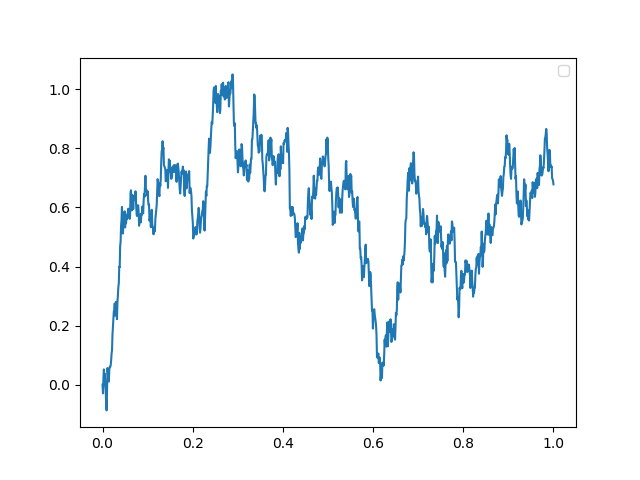
\includegraphics[width=6cm,height=4cm]{Figure_1.png}\\
\centering	
\end{figure}
\subsection{其他随机过程}
模拟随机过程
\begin{equation}
u(W(t))=\exp \left(t+\frac{1}{2} W(t)\right)
\end{equation}
$u(W(t))$的均值为$e^{9t/8}$,重复试验4000次求其均值,结果如下
\begin{figure}[H]
	\centering
	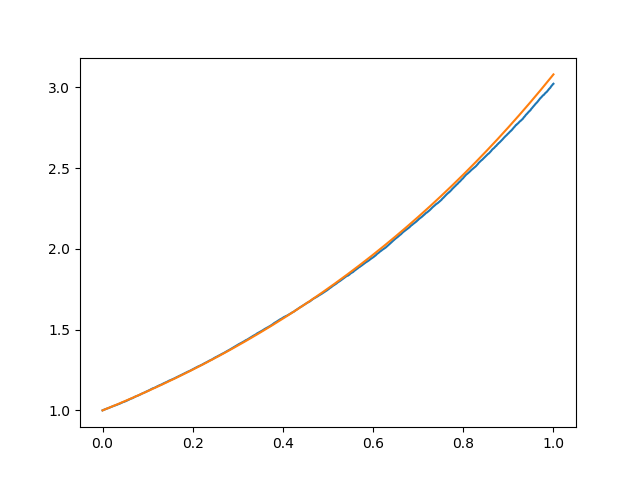
\includegraphics[width=6cm,height=4cm]{Figure_2.png}\\
	\centering	
\end{figure}



\end{document}